%!TEX root = alga.tex
\section{Algebraic structure}\label{sec-algebra}

The functions \hs{edge}, \hs{vertices} and \hs{clique} defined in the previous
section \S\ref{sec-core} satisfy a few properties that we can intuitively write down,
but which may seem tricky to prove (we encourage the reader to try):
\begin{itemize}
    \item \hs{vertex x} $\ =\ $ \hs{vertices [x]} and \hs{edge x y} $\ =\ $ \hs{clique [x,y]}.
    \item \hs{vertices xs} $\ \subseteq\ $ \hs{clique xs}, where $x \subseteq y$ means
    $x$ is a subgraph of $y$.
    \item \hs{clique (xs ++ ys)} $\ =\ $ \hs{connect (}\hs{clique xs) (}\hs{clique ys)}.
\end{itemize}

In this section we characterise the \hs{Graph} type class with a set of
axioms that reveal an algebraic structure very similar to a semiring\footnote{
See~\citet{1999_semirings_golan} for a classic overview of semiring
applications. \citet{2013_semirings_dolan} uses the semiring theory
to implement graph algorithms.}.
This provides a convenient framework for proving graph properties, such as
those listed above, using equational
reasoning. The presented characterisation is generally useful for formal
verification, as well as automated testing
of graph library APIs, e.g. by using QuickCheck~\cite{2011_quickcheck_claessen}.

\begin{figure}
\begin{subfigure}[b]{0.4\linewidth}
\centerline{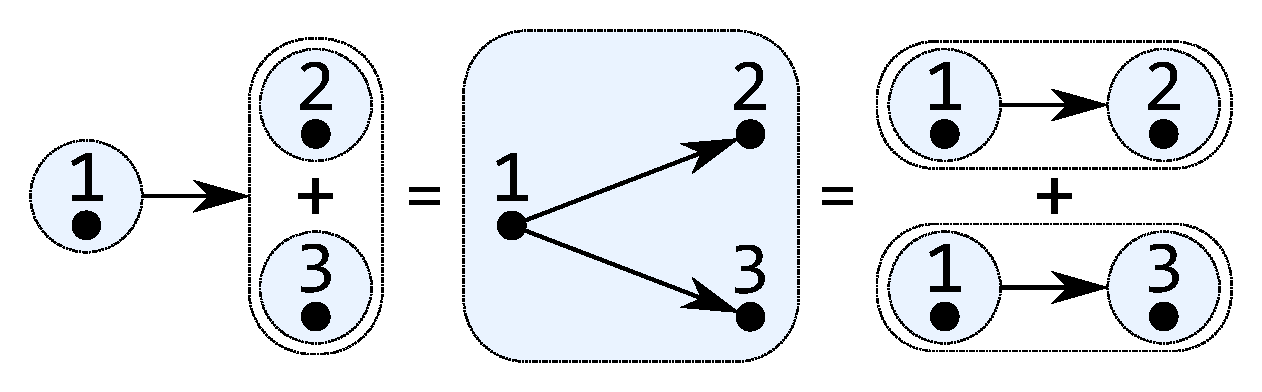
\includegraphics[scale=0.27]{fig/ax-distributivity.pdf}}
\caption{Distributivity: $1 \rightarrow (2 + 3) = 1 \rightarrow 2 + 1 \rightarrow 3$ }
\end{subfigure}
\hspace{12mm}
\begin{subfigure}[b]{0.5\linewidth}
\centerline{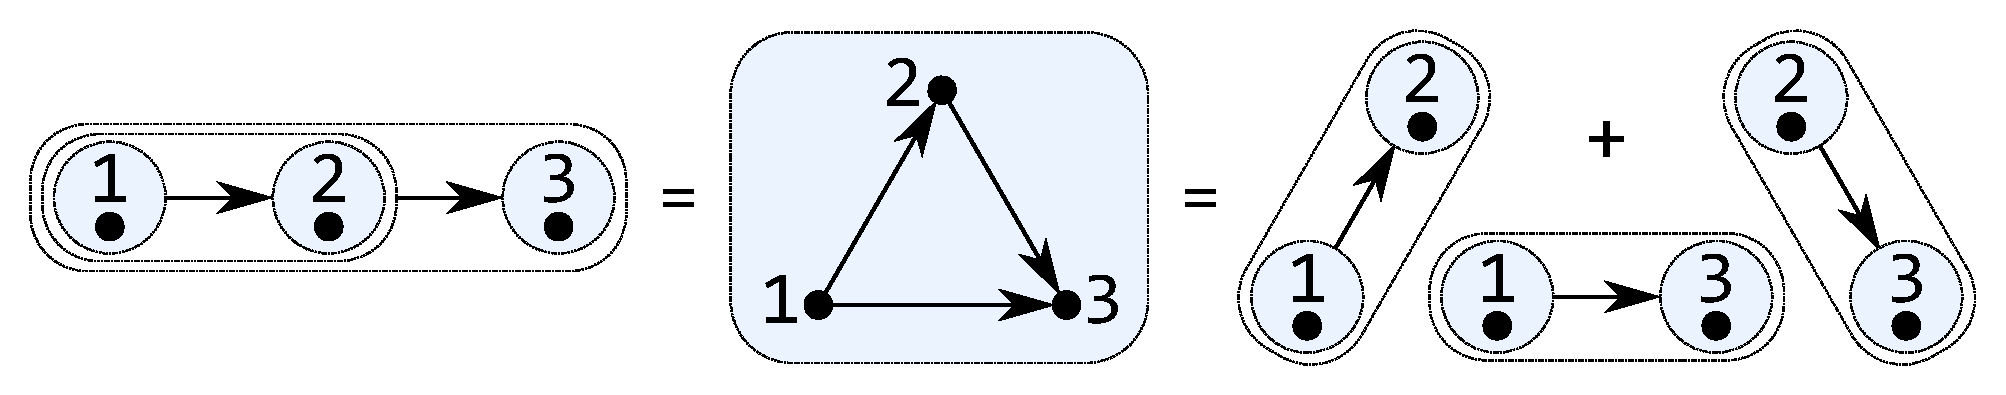
\includegraphics[scale=0.27]{fig/ax-decomposition.pdf}}
\caption{Decomposition: $1 \rightarrow 2 \rightarrow 3 = 1 \rightarrow 2 +
1 \rightarrow 3 + 2 \rightarrow 3$}
\end{subfigure}
\vspace{-3mm}
\caption{Two axioms of the algebra of graphs\label{fig-axioms}}
\vspace{-4mm}
\end{figure}

\subsection{Axiomatic characterisation}\label{sub-laws}

The definitions of \hs{vertices} and \hs{clique} in \S\ref{sub-class}
use $\varepsilon$ as the identity for both overlay $+$ and connect $\rightarrow$
operations. This seems unusual, but we can easily check that
$x + \varepsilon = x$ and $x \rightarrow \varepsilon = x$ for any graph $x \in G$
by plugging the empty graph into the definitions of overlay and connect,
respectively. Furthermore, we can verify the following:
\begin{itemize}
    \item $(G,+,\varepsilon)$ is an idempotent commutative monoid.
    \item $(G,\rightarrow,\varepsilon)$ is a monoid.
    \item $\rightarrow$ distributes over $+$, e.g.
    $1 \rightarrow (2 + 3) = 1 \rightarrow 2 + 1 \rightarrow 3$, as illustrated
    in Fig.~\ref{fig-axioms}(a).
\end{itemize}

\noindent
The above looks remarkably close to a semiring, with the only oddity being the shared
identity of the two operations. The following \emph{decomposition} law is
what makes the algebra of graphs different:
\[
x \rightarrow y \rightarrow z = x \rightarrow y + x \rightarrow z + y \rightarrow z
\]

\noindent
Fig.~\ref{fig-axioms}(b) illustrates the law by showing that the triangle
graph can be obtained in two different ways: by connecting three vertices
of the triangle or by constructing its edges separately and overlaying them.

Interestingly, the fact that overlay and connect share the same identity
follows from the decomposition law. Indeed, let $\varepsilon_{+}$ and
$\varepsilon_{\rightarrow}$ stand for the identities of $+$ and $\rightarrow$,
respectively. Then:
\[
\begin{array}{rcll}
\varepsilon_{+} & = & \varepsilon_{+} \rightarrow \varepsilon_{\rightarrow} \rightarrow \varepsilon_{\rightarrow} & \text{(identity of $\rightarrow$)}\\
 & = & \varepsilon_{+} \rightarrow \varepsilon_{\rightarrow} + \varepsilon_{+} \rightarrow \varepsilon_{\rightarrow} + \varepsilon_{\rightarrow} \rightarrow \varepsilon_{\rightarrow} & \text{(decomposition)}\\
 & = & \varepsilon_{+} + \varepsilon_{+} + \varepsilon_{\rightarrow} & \text{(identity of $\rightarrow$)}\\
 & = & \varepsilon_{\rightarrow} & \text{(identity of $+$)}\\
\end{array}
\]

\noindent
Furthermore, the idempotence of $+$ can also be proved from the decomposition, which
leads to the following \emph{minimal set of axioms that characterise algebraic graphs}:

\begin{itemize}
    \item $+$ is commutative and associative: $x + y = y + x$ and
    $x + (y + z) = (x + y) + z$.
    \item $(G, \rightarrow, \varepsilon)$ is a monoid:
    $\varepsilon \rightarrow x = x \rightarrow \varepsilon = x$ and
    $x \rightarrow (y \rightarrow z) = (x \rightarrow y) \rightarrow z$.
    \item Distributivity:
    $x \rightarrow (y + z) = x \rightarrow y + x \rightarrow z$ and
    $(x + y) \rightarrow z = x \rightarrow z + y \rightarrow z$.
    \item Decomposition: $x \rightarrow y \rightarrow z =
    x \rightarrow y + x \rightarrow z + y \rightarrow z$.
\end{itemize}

We require all \hs{Graph} instances to satisfy these 8 axioms. Our definition
of graph construction primitives in~\S\ref{sub-constructing} does satisfy them
all and is therefore a valid \hs{Graph} instance. We will provide an
implementation for this and other useful instances in~\S\ref{sec-a-la-carte}.
Some of them will satisfy additional
axioms, for example, by making the connect $\rightarrow$ operation commutative,
we obtain undirected graphs.

Algebraic graphs are \emph{complete} in the sense that it is possible to describe
any graph using the core interface. Indeed, given a graph $(V,E)$ we can construct
it as \hs{graph@$\,V\,E$@}, where the function \hs{graph} is defined as follows.

\begin{minted}{haskell}
graph :: Graph g => [Vertex g] -> [(Vertex g, Vertex g)] -> g
graph vs es = overlay (vertices vs) (edges es)
\end{minted}

Here \hs{edges} is a generalisation of \hs{edge} to a list of edges, so that
\hs{edge x y} $\ =\ $ \hs{edges [(x,y)]}:

\begin{minted}{haskell}
edges :: Graph g => [(Vertex g, Vertex g)] -> g
edges = @\std{foldr}@ overlay empty . @\std{map}@ (@\std{uncurry}@ edge)
\end{minted}

Note that \hs{graph} is total thanks to the \emph{absorption theorem}
$x \rightarrow y + x + y = x \rightarrow y$, which in particular states that
an edge $(u,v)$ contains its two vertices $\{u,v\}$ and is inseparable
from them. Therefore, if the pair $(V,E)$ is inconsistent, the set of vertices of
the resulting graph will be expanded to $\hat{V}$ so that
$E\subseteq \hat{V}\times \hat{V}$ holds. More generally, the absorption
theorem states that in addition to being complete, the algebraic graph
API is also \emph{sound} in the sense that it is impossible to construct
an inconsistent pair $(V,E)$ using the four \hs{Graph} methods.

The following theorems can be proved from the minimal set of axioms:

\begin{itemize}
    \item Identity of $+$: $x + \varepsilon = x$.
    \item Idempotence of $+$: $x + x = x$.
    \item Absorption: $x \rightarrow y + x + y = x \rightarrow y$.
    \item Saturation: $x \rightarrow x \rightarrow x = x \rightarrow x$.
\end{itemize}

We leave the proof to the reader as a not entirely trivial exercise.
\citet{2014_alekseyev_phd} formalised the algebra of
parameterised graphs (that we build on) in Agda and derived a
machine-assisted proof of these theorems.

\subsection{Partial order on graphs}\label{sub-partial-order}

It is fairly standard to define $x \preceq y$ as $x + y = y$ for an
idempotent $+$ operation, since it gives a partial order on the elements
of the algebra. Indeed, all partial order laws are satisfied:

\begin{itemize}
     \item Reflexivity $x \preceq x$ follows from the idempotence $x + x = x$.
     \item Antisymmetry $x \preceq y \wedge y \preceq x \Rightarrow x = y$ holds
     since $x + y = y$ and $y + x = x$ imply $x = y$.
     \item Transitivity $x \preceq y \wedge y \preceq z \Rightarrow x \preceq z$
     can be proved as $z = y + z = (x + y) + z = x + (y + z) = x + z$.
 \end{itemize}

\noindent
It turns out that this definition corresponds to the \emph{subgraph} relation,
i.e. we can define:
\[
x \subseteq y~~\defeq~~x + y = y.
\]

\noindent
Indeed, expanding $x + y = y$ to $(V_x,E_x) + (V_y,E_y) = (V_y,E_y)$ gives us
$V_x \cup V_y = V_y$ and $E_x \cup E_y = E_y$, which is equivalent to
$V_x \subseteq V_y$ and $E_x \subseteq E_y$, as desired.

Therefore, we can check if a graph is a subgraph of another one if we know how to
compare graphs for equality:
\begin{minted}{haskell}
isSubgraphOf :: (Graph g, Eq g) => g -> g -> Bool
isSubgraphOf x y = overlay x y == y
\end{minted}

The following theorems about the partial order on graphs can be proved:

\begin{itemize}
    \item Least element: $\varepsilon \subseteq x$.
    \item Overlay order: $x \subseteq x + y$.
    \item Overlay-connect order: $x + y \subseteq x \rightarrow y$.
    \item Monotony: $x \subseteq y \Rightarrow (x + z \subseteq y + z)
    \wedge (x \rightarrow z \subseteq y \rightarrow z)
    \wedge (z \rightarrow x \subseteq z \rightarrow y)$.

\end{itemize}

\subsection{Equational reasoning}\label{sub-reasoning}

In this subsection we show how to use equational reasoning and the laws
of the algebra to prove properties of functions on graphs.
For example, let's prove that \hs{vertex x} $=$ \hs{vertices [x]} by rewriting
the right-hand side:
\[
\begin{array}{rcll}
\hs{vertices [x]} & = & \hs{@\std{foldr}@ overlay empty (@\std{map}@ vertex [x])} & \text{(definition of \hs{vertices})}\\
 & = & \hs{@\std{foldr}@ overlay empty [vertex x]} & \text{(definition of }\hs{@\std{map}@}\text{)}\\
 & = & \hs{overlay (vertex x) empty} & \text{(definition of }\hs{@\std{foldr}@}\text{)}\\
 & = & \hs{vertex x} & \text{(overlay identity)}\\
\end{array}
\]

Proving that \hs{vertices xs} $\ \subseteq\ $ \hs{clique xs} requires more work.
We start with the case when $\hs{@\blk{xs}@}$ is the empty list $\hs{[@@]}$,
which is straightforward:
$\hs{vertices [@@]} = \varepsilon \subseteq \varepsilon = \hs{clique [@@]}$,
as follows from the definition of \hs{@\std{foldr}@}.
If $\hs{@\blk{xs}@}$ is non-empty, i.e. $\hs{@\blk{xs}@}\ =\ \hs{@\blk{h}@:t}$,
we make the inductive hypothesis (*) that
\hs{vertices t} $\ \subseteq\ $ \hs{clique t} and proceed as follows:
\[
\begin{array}{rcll}
\hs{vertices (h:t)} & = & \hs{@\std{foldr}@ overlay empty (@\std{map}@ vertex (h:t))} & \text{(definition of \hs{vertices})}\\
 & = & \hs{@\std{foldr}@ overlay empty (vertex h : @\std{map}@ vertex t)} & \text{(definition of }\hs{@\std{map}@}\text{)}\\
 & = & \hs{overlay (vertex h) (vertices t)} & \text{(definition of }\hs{@\std{foldr}@}\text{)}\\
 & \subseteq & \hs{overlay (vertex h) (clique t)} & \text{(monotony and *)}\\
 & \subseteq & \hs{connect (vertex h) (clique t)} & \text{(overlay-connect order)}\\
 & = & \hs{@\std{foldr}@ connect empty (vertex h : @\std{map}@ vertex t)} & \text{(definition of }\hs{@\std{foldr}@}\text{)}\\
 & = & \hs{@\std{foldr}@ connect empty (@\std{map}@ vertex (h:t))} & \text{(definition of }\hs{@\std{map}@}\text{)}\\
 & = & \hs{clique (h:t)} & \text{(definition of \hs{clique})}\\
\end{array}
\]

\noindent
This completes our proof: \hs{vertices xs} $\ \subseteq\ $ \hs{clique xs}
holds in all possible cases.

\begin{figure}[b]
\vspace{-2mm}
\begin{subfigure}[b]{0.48\linewidth}
\begin{minted}{haskell}
gen ::@\,@(Graph g,@\,@Arbitrary@\,@(Vertex g)) => Gen g
gen = sized expr
  where
    expr 0 = @\std{return}@ empty
    expr 1 = @\std{fmap}@ vertex arbitrary
    expr n = do
        sizeLeft <- choose (0, n)
        l <- expr sizeLeft
        r <- expr (n - sizeLeft)
        elements [ overlay l r, connect l r ]

instance Arbitrary a => Arbitrary@\,@(Expr@\,@a) where
    arbitrary = gen

    shrink Empty = []
    ...
\end{minted}
\caption{Generating arbitrary algebraic graphs}
\end{subfigure}
\hfill
\hfill
\hfill
\vrule
\hfill
\begin{subfigure}[b]{0.45\linewidth}
\begin{minted}{haskell}
(+) = overlay -- convenient shortcuts
(*) = connect

type GraphTestsuite g = (Eq g, Graph g)
  => g -> g -> g -> Property

axioms :: GraphTestsuite g
axioms x y z = conjoin
  [       x + y == y + x
  , x + (y + z) == (x + y) + z
  ,   empty * x == x
  ,   x * empty == x
  , x * (y * z) == (x * y) * z
  , x * (y + z) == x * y + x * z
  , (x + y) * z == x * z + y * z
  ,   x * y * z == x * y + x * z + y * z ]
\end{minted}
\caption{Testsuite for the minimal set of axioms}
\end{subfigure}
\vspace{-3mm}
\caption{Automated testing infrastructure for algebraic graphs\label{fig-testing}}
\end{figure}

\subsection{Automated testing}\label{sub-testing}

Theorem provers, such as Agda~\cite{2007_norell_agda},
can substantially reduce the effort required for formal verification,
however, automated testing remains an effective and pervasively used
method for formulating and testing functional properties. In Haskell,
the go-to tool for automated testing is QuickCheck developed
by~\citet{2011_quickcheck_claessen}.
Fig.~\ref{fig-testing} shows a reusable testing infrastructure for
algebraic graphs. The function~\hs{gen} in Fig.~\ref{fig-testing}(a)
allows to generate arbitrary graph expressions of specified size.
It is polymorphic and can therefore be used as a default implementation
of QuickCheck's \hs{Arbitrary} type class, as shown by a sketch of
the \hs{Arbitrary@\,\,@(Expr@\,\,\blk{a}@)} instance definition, where \hs{Expr}
is a \hs{Graph} instance defined in the next section~\S\ref{sec-a-la-carte}.

Fig.~\ref{fig-testing}(b) shows an implementation of the \hs{axioms}
testsuite that can be used for testing a \hs{Graph} instance against
the minimal set of axioms defined in~\S\ref{sub-laws}.
For example, let's do a quick check of \hs{Expr@\,@Int} in the interactive GHC:

\begin{minted}[frame=single]{haskell}
@\ghci @quickCheck (axioms :: GraphTestsuite (Expr Int))
@\blk{+++ OK, passed 100 tests.}@
\end{minted}

\noindent
Here QuickCheck generates 100 random test cases $(x,y,z)$ using the \hs{gen}
function and checks that \hs{axioms@\,$x\,y\,z$@} holds in each case. Note
that we have to tell QuickCheck which specific \hs{Graph} instance to test
by providing a type signature for the polymorphic \hs{axioms} testsuite.

Finally, let's use QuickCheck to test the property
\hs{clique (xs ++ ys)} $\ =\ $ \hs{connect (}\hs{clique xs) (}\hs{clique ys)},
which we contemplated in the beginning of this section:

\begin{minted}[frame=single]{haskell}
@\ghci @quickCheck $ \xs ys -> clique@\,@(xs ++ ys) == connect@\,@(clique xs) (clique ys :: Epxr Int)
@\blk{+++ OK, passed 100 tests.}@
\end{minted}

\noindent
All properties and theorems that we discuss (and occasionally \hs{quickCheck})
have been formally proved in Agda.
